\documentclass[a4paper,11pt]{article}
\usepackage[czech]{babel}
\usepackage{amsmath, amssymb, listings}
\usepackage[T1]{fontenc}
\usepackage[utf8]{inputenc}
\usepackage{hyperref}
\usepackage{graphicx}
\usepackage{geometry}
\usepackage{todonotes}
\usepackage{longtable}
\usepackage{xcolor}
\usepackage{csquotes}
\geometry{a4paper, margin=1in}

\newcommand{\nepovedeno}{\protect\textbf{\protect\color{red}(Neúspěšný pokus)}}
\newcommand{\povedeno}{\protect\textbf{\protect\color{green}(Úspěšný pokus)}}
\newcommand{\moznost}{\protect\textbf{\protect\color{orange}(Možná cesta)}}

\setlength{\parskip}{0.7\baselineskip}
\setlength{\parindent}{0pt}
\setlength{\marginparwidth}{2cm}

\newcommand{\ukol}[1]{\todo[inline]{#1}}


\usepackage[backend=biber,style=iso-numeric]{biblatex}
\addbibresource{references.bib} 

\begin{document}
\listoftodos

\newpage

\begin{titlepage}
    \centering
    
\includegraphics[width=0.4\textwidth]{assets/PřF-UJEP-logo.png}
    
        \vfill
    
    {\LARGE Univerzita Jana Evangelisty Purkyně v Ústí nad Labem}\\[1.5cm]
    {\huge \bfseries Konfigurace Mellanox ConnectX-5 v Proxmox virtualizaci\\}
    
    \vfill
    \begin{flushleft}
        \large
        \textbf{Autoři:} \\
        Bao Kieu Quang, Jakub Petrášek, Martin Kopecký\\[1cm]

        \textbf{Vypracováno:} 5. března 2025 \\
        \textbf{Upraveno:} \today 
    \end{flushleft}
    
\end{titlepage}

\newpage

\tableofcontents


\newpage
\section{Úvod}
Úkolem práce je zprovoznění komunikace 100Gbps karty Mellanox ConnectX-5 pod operačním systémem Proxmox. Komunikace bude probíhat přes 
Mellanox SB7790 InfiniBand switch, který podporuje komunikaci pouze přes protokol InfiniBand\cite{InfiniBand}. Linuxové platformy nemají vestavěné ovladače v jádře.
\newpage

\section{Rozdíly mezi Ethernetem a InfiniBand}
Ethernet a InfiniBand\cite{InfiniBand} jsou dvě odlišné technologie pro síťovou komunikaci, které se liší v několika klíčových aspektech:
\begin{itemize}
    \item \textbf{Protokolová architektura} – Ethernet využívá TCP/IP model s vrstvovou strukturou, zatímco InfiniBand\cite{InfiniBand} je nízkoúrovňová síťová technologie orientovaná na vysokou propustnost a nízkou latenci.
    \item \textbf{Latence} – InfiniBand\cite{InfiniBand} nabízí extrémně nízkou latenci v řádu mikrosekund, zatímco běžné Ethernet sítě mají latence v řádu milisekund.
    \item \textbf{Propustnost} – InfiniBand\cite{InfiniBand} podporuje přenosové rychlosti až 400 Gb/s, což je výrazně více než u standardních Ethernet sítí.
    \item \textbf{Síťová topologie} – Ethernet sítě jsou obvykle hierarchicky uspořádané s využitím přepínačů a směrovačů, zatímco InfiniBand\cite{InfiniBand} umožňuje přímou komunikaci mezi uzly pomocí RDMA (Remote Direct Memory Access).
    \item \textbf{Použití} – Ethernet je dominantní v tradičních podnikových sítích, zatímco InfiniBand\cite{InfiniBand} se používá zejména v HPC (High-Performance Computing) a datových centrech.
\end{itemize}
\newpage

\section{Hledání řešení}

\subsection{Pokus 1) Proxmox 8.3.1 + Nvidia MLNX-EN}
\label{pokus1}
\nepovedeno

Jako první jsme zkoušely nainstalovat nejnovější verzi platformy Proxmox jest je verze 8.3.1 (Debian 12.9). Dále jsme pokračovaly podle návodu co nám poskytla umělá inteligence. To tím že jsem chtěly nainstalovat ovladače MLNX-EN\cite{EN}.

\subsubsection{Nález}
Ovladače Nvidia MLNX-EN\cite{EN} nelze nainstalovat na Debian 12.9. Proto jsme byly nuceni přejít na starší verzi platformy Proxmox a to jest Proxmox 8.2.2 (Debian 12.5).




\subsection{Pokus 2) Proxmox 8.2.2 + Nvidia MLNX-EN}
\label{pokus2}
\nepovedeno

Po zjištění že verze 8.2.2 má jádro Debian 12.5 jsme přeinstalovaly celý systém na tuto verzi. Dále jsme stáhly ovladače a daly je instalovat. Při instalaci se nainstalovaly ovladače a aktualizoval Firmware sítových karet Mellanox ConnectX-5. Vše proběhlo v pořádku. Jenže po doinstalovaní se karta stále neobjevovala jako síťová. Po dohledávání v dokumentaci jsme se  dozvěděly že kartu lze softwarově přepnout do režimu Ethernet a hned poté se objevila, ale v tento moment jsme zjistily že switch nepodporuje Ethernet mód a tudíž je nutno najít způsob jak zprovoznit InfiniBand\cite{InfiniBand} a IP over InfiniBand (IPoIB)\cite{IPoIB}.

\subsubsection{Nález}
V jádře systému nejsou InfiniBand ovladače a schází podpora pro IP over InfiniBand.

\subsection{Pokus 3) Proxmox 8.2.2 + Nvidia MLNX-EN + IB}
\label{pokus3}
\nepovedeno

Dále pokračovala snaha o zprovoznění síťové karty po nalezení Open-Source ovladačů pro ovládání InfiniBand\cite{InfiniBand}. Přesněji ovladačů RDMA\cite{guideDeb} (rdma\_core). Instalace proběhla podle návodu\cite{guideDeb}, ale i po této snaze karta stále nebyla rozpoznána.

Pro instalaci byly použity tyto komandy
\begin{verbatim}
    apt install rdma-core
    apt install libibverbs1 librdmacm1 \
libibmad5 libibumad3 librdmacm1 ibverbs-providers rdmacm-utils \
infiniband-diags libfabric1 ibverbs-utils
\end{verbatim}

\subsubsection{Nález}
Při delší prohledávání internetu jsme se dozvěděly, že MLNX-EN\cite{EN} nejsou ovladače pro InfiniBand ale pro Ethernet. Proto jsem musely přeinstalovat systém a začít znovu.

\subsection{Pokus 4) Proxmox 8.2.2 + Nvidia MLNX-OFED + IB}
\label{pokus4}
\nepovedeno

Další snaha byla převést ovladače Nvidia MLNX-EN\cite{EN} na MLNX-OFED\cite{OFED}, které jsou určeny pro RDMA\cite{RDMA} mód. Jenže při instalaci vyskočila chybová hláška, která nám oznámila že je třeba odinstalovat balíček proxmox-ve, který je nutný pro chod systému.

\subsubsection{Nález}
Ovladače MLNX-OFED\cite{OFED} nejsou kompatibilní s platformou Proxmox. Pro její zprovoznění by bylo nutno nainstalovat čistý Debian 12.5 a manuálně jej převést na Proxmox platformu.

\subsection{Pokus 5) Proxmox 8.2.2 + IB}
\label{pokus5}
\nepovedeno

Po delším hledání jsme nalezly uživatele Alpha75429 na  Proxmox fóru, který řešil ten samý problém před námi. Díky jeho příspěvku\cite{guide} jsme byly schopni zprovoznit síťovou kartu aby byla detekována a to jest instalací jen Open-source ovladačů.

instalace ovladačů
\begin{verbatim}
apt install -y infiniband-diags opensm ibutils rdma-core rdmacm-utils
\end{verbatim}

zavedení ovladačů do jádra
\begin{verbatim}
modprobe ib_umad
modprobe ib_ipoib
\end{verbatim}

nutná kontrola detekce síťové karty.
\begin{verbatim}
ip link show 
\end{verbatim}

nastavení statické IP adresy a to přidáním do souboru \texttt{/etc/network/interfaces} konfigurace \texttt{ib0}:
\begin{verbatim}
auto ibs1
iface ibs1 inet static
    address 10.0.0.1
    netmask 255.255.255.0
    mtu 2044
\end{verbatim}

Aplikace síťových změn
\begin{verbatim}
systemctl restart networking
\end{verbatim}


Ověření funkce IPoIB mezi dvěma servery
\begin{verbatim}
apt install iperf3 -y

# nodeA
iperf3 -s

# nodeB
iperf3 -c 10.0.0.2
\end{verbatim}

\subsubsection{Nález}
Bohužel po zprovoznění IPoIB jsme nalezly rychlosti jen 20Gbps při syntetickém testování. Proto jsem přesunuly dva systémy na Rocky9.5 pro možnost instalování MLNX-OFED\cite{OFED}. IPoIB je stále potencionální možnost jestli že budeme schopni dostat MTU do řádu 65000.

Při testování v rámci platformy Proxmox VE a CEPH jsme se dostaly jen na 2Gbps až 2,5Gbps. Konečná limitace je chod Proxmox VE a CEPH přes TCP/IP což je velice limitováno při použití IPoIB. CEPH ani Proxmox VE nativně nepodporují InfiniBand

\newpage
\subsection{Pokus 6) Rocky9.5 + DOCA\_OFED + IB}
\label{pokus6}
\povedeno

Po nainstalovaní jsme se pustily do instalace Nvidia DOCA\_OFED ovladačů. Po jejich instalaci jsme byly překvapeni těmito výsledky.

Výsledky jsou při čtení v módu RDMA
\begin{footnotesize}
\begin{verbatim}
[root@localhost ~]# ib_read_bw -d mlx5_0

************************************
* Waiting for client to connect... *
************************************
---------------------------------------------------------------------------------------
                    RDMA_Read BW Test
 Dual-port       : OFF		Device         : mlx5_0
 Number of qps   : 1		Transport type : IB
 Connection type : RC		Using SRQ      : OFF
 PCIe relax order: ON		Lock-free      : OFF
 WARNING: CPU is not PCIe relaxed ordering compliant.
 WARNING: You should disable PCIe RO with `--disable_pcie_relaxed` for both server and client.
 ibv_wr* API     : ON		Using DDP      : OFF
 CQ Moderation   : 1
 Mtu             : 4096[B]
 Link type       : IB
 Outstand reads  : 16
 rdma_cm QPs	 : OFF
 Data ex. method : Ethernet
---------------------------------------------------------------------------------------
 local address: LID 0x04 QPN 0x0028 PSN 0xceaff0 OUT 0x10 RKey 0x1fff00 VAddr 0x007ff0816d9000
 remote address: LID 0x05 QPN 0x0028 PSN 0xa27746 OUT 0x10 RKey 0x1fff00 VAddr 0x007f7429027000
---------------------------------------------------------------------------------------
 #bytes     #iterations    BW peak[MiB/sec]    BW average[MiB/sec]   MsgRate[Mpps]
 65536      1000             10629.15            10628.79		     0.170061
---------------------------------------------------------------------------------------
\end{verbatim}

\end{footnotesize}

Tato rychlost je dosažitelná pouze přes InfiniBand \cite{InfiniBand}.

\subsubsection{Nález}
Byla dosažena rychlost 90Gbps až 92Gbps při syntetickém testu v rámci konektivity přes IB a při použití testování rychlosti přes Iperf rychlosti se pohybovaly okolo 82Gbps.

\newpage

\subsection{Pokus 7) FreeBSD}
\label{pokus7}
\nepovedeno

FreeBSD nemá nativní podporu pro OFED ani EN ovladače od Nvidia. Veškerá implementace závisí na komunitě. Syntetické testy ukázaly rychlosti v řádu 5Gb/s. Pro instalaci byl použit návod\cite{OFEDBSD} z platformy Github.

\subsubsection{Nález}
Implementace IPoIB je horší než na linux platformách.


\subsection{Pokus 8) Debian 12.9 + DOCA-ALL}
\label{pokus8}
\nepovedeno

Další pokus byl s použitím DOCA\cite{DOCA} ovladačů. Po nainstalování se interface síťové karty neobjevil a byl zjištěn problém že ovladače nelze použít v režimu IPoIB.

\subsubsection{Nález}
Ovladače DOCA\cite{DOCA} nejsou použitelné pro náš účel.

\subsection{Pokus 9) RedHat + CentOS10 + Eth mód}
\label{pokus9}
\nepovedeno

Při přepnutí karty do Eth módu a přímém připojení byla dosažena rychlost 40Gbps. Problém nastává že nemáme k dispozici switch s QSFP28 a Eth módem.

\subsection{Pokus 10) CentOS10 + MLNX\_OFED}
\label{pokus10}
\povedeno

Instalace OFED ovladačů přinesla konečně úspěch a to tím že konečně byla dosažena rychlost okolo 100Gbps (přesněji 89Gbps). Dosáhly jsme tak při použití starých ovladačů od Nvidia a to poslední LTS build MLNX\_OFED. Nainstalovány byly jen OFED ovladače a test byl přes iperf3.

Systém byl nainstalován bez podpory pro InfiniBand. Ta byl následně doinstalována za pomocí Nvidia MLNX\_OFED ovladačů.

\newpage
\subsection{Pokus 11) Windows Server 2025 + MLNX\_WinOF2}
\label{pokus11} 
\nepovedeno

\paragraph{Instalace Windows Server 2025}  
Operační systém Windows Server 2025 byl úspěšně nainstalován na obě testovací stanice bez komplikací.

\paragraph{Instalace ovladačů MLNX\_WinOF2}  
Po instalaci oficiálního balíčku \texttt{MLNX\_WinOF2} došlo ke komplikacím: síťové rozhraní bylo sice detekováno jako \texttt{Mellanox ConnectX-5}, avšak příslušná služba \texttt{MellanoxNDProvider} nebyla aktivní. Služba sice existovala v systému, ale nebyla spustitelná z důvodu chybějících binárních souborů, konkrétně \texttt{mlnxnd.sys}. Pokus o ruční spuštění selhal s chybou \texttt{Cannot start service MellanoxNDProvider... The system cannot find the file specified}.  

Dále bylo zjištěno, že základní instalace neobsahuje testovací a konfigurační nástroje jako \texttt{ib\_send\_bw.exe}, \texttt{mlxconfig.exe}, či \texttt{flint.exe}, a není ani součástí balíčku MFT. Tyto nástroje je nutné doinstalovat samostatně z oficiální stránky NVIDIA Networking.

\paragraph{Instalace a testování WinMFT}  
Po instalaci nástroje WinMFT (verze 4.22.1.406 – kompatibilní s ConnectX-5) se stále nevytvořila složka \texttt{bin}, která je pro provoz některých nástrojů nezbytná. Bylo zjištěno, že balíčky dostupné na oficiální stránce často neobsahují plnou sadu nástrojů, případně chybí správná konfigurace služby MST.

Po ruční registraci služby \texttt{MellanoxNDProvider} a jejím pokusu o spuštění systém nadále hlásil absenci potřebného ovladače.

\subsubsection{Zjištění}
Po částečné konfiguraci byla síťová karta přepnuta do režimu InfiniBand, což bylo ověřeno pomocí nástroje \texttt{mlxconfig} (po aktivaci \texttt{mst status}). Přesto však nebylo možné využít benchmarkingové nástroje jako \texttt{ib\_send\_bw}, protože jejich spustitelné soubory v systému chyběly. Pokus o využití WSL (Windows Subsystem for Linux) a instalaci balíku \texttt{OFED} selhal, neboť Mellanox/OFED není ve WSL plně podporován.

\subsubsection{Závěr}  
Na systému Windows Server 2025 se ukázalo jako problematické provozovat InfiniBand benchmarky. Chybějící binární soubory, nekompletní balíčky nástrojů a chybová inicializace služeb bránily provedení testů propustnosti. Pro správné testování je doporučeno přejít na Linuxové prostředí s plnohodnotným OFED stackem nebo využít Mellanox nástroje na LiveCD distribuci od NVIDIA (např. UFM bootable image).

\newpage
\subsection{Pokus 12) Harvester virtualizace na SUSE Linux}
\nepovedeno

Instalace systému a ovladačů úspěšná. Ping na jiný systém pomocí InfiniBand úspěšný. Systém je nevhodný pro nasazení z důvodu, že to je \textit{immutable system}. Z tohoto důvodu je systém pouze read only a musí se přepnout v grubu do debug modu. Po restartováné si Harvester smaže konfigurační složky spojené s konfigurací IB interfacu. Dále je obtížné dohledávání repozitářů pro jakoukoliv následnou instalaci. Například nebyla otestovaná rychlost spojení přes IB.

Možný další pokus s nainstalováním SUSE a nastavením, poté doinstalace Harvesteru. Zatím jsem nenašel návod na internetu.

\section{Výsledky hledání}

\subsection{Tabulka výsledků testování}
\begin{center}
    
\begin{tabular}{|c|c|c|c|c|c|}
    \hline
    \textbf{OS} &
    \textbf{Ovladače} &
    \textbf{Metoda} &
    \textbf{IB rychl.} &
    \textbf{IPoIB rychl.} \\
    \hline
Proxmox 8.3.x & MLNX\_OFED   & -   & - & -  \\
\hline
Proxmox 8.3.x & MLNX\_EN   & -   & - & -  \\
\hline
Proxmox 8.3.x & OSS RDMA + IB   & IPoIB & - & 20Gbps \\
\hline
Proxmox 8.2.1 & MLNX\_OFED   & IB & - & -   \\
\hline
Proxmox 8.2.1 & MLNX\_EN     & Eth & - & - \\
\hline
Proxmox 8.2.1 & OSS RDMA + IB   & IPoIB & - & 20Gbps  \\
\hline
\textbf{Rocky 9.5} & MLNX\_OFED & IB & 92Gbps & 82Gbp  \\
\hline
FreeBSD 14.2 & OSS IB & IPoIB & - & 5Gbps  \\
\hline
Debian 12.9 & DOCA-ALL & IB & - &  -  \\
\hline
CentOS s. 10 & DOCA\_OFED & IPoIB & 91Gbps &  89Gbps  \\
\hline
\textbf{CentOS s. 9} & DOCA\_OFED & IPoIB & 90Gbps &  60Gbps  \\
\hline
\end{tabular}
\end{center}

\subsection{Zvolené řešení}

Pro finální nasazení pro platformu OpenNebula byly zvoleny \textbf{Centos Stream 9} a \textbf{RockyLinux 9.5}. Důvodem pro volbu těchto Linux distribucí je rychlost komunikace přes protokol IPoIB\cite{IPoIB} a podpora samotné síťové implementace pro InfiniBand\cite{InfiniBand} a IPoIB\cite{IPoIB}. 
\newpage

\section{Instalace OpenNebula na RockyLinux 9.5}

\subsection{Základní informace}

Pro tento postup je nutno dodat základní informace zápisu. V příkazových blocích budou značení použití s pravomocemi.

\begin{large}
Značení práv příkazu    
\end{large}

\textbf{\#} administrátorská pravá

\textbf{\$} uživatelské pravá


\subsection{Úvod}

Nutno nainstalovat čistý systém RockyLinux 9.5 v server módu bez žádných balíčků z výběru. Dále budou použity automatizační nástroje pro instalaci ovladačů a základní nastavení. Na \url{https://github.com/KopyTKG/UJEP-LAB} lze najít již předepsané nástroje. 

Pro pokračování budeme předpokládat že systémy Supermicro BMC, BIOS/EUFI a firmware síťové karty byly již aktualizovány na nejnovější možnou verzy.

\newpage

\subsection{Logické zapojení sítě}
Na diagramu lze vidět logické zapojení sítě. Našeb topologie obsahuje 2 oddělené sítě a to jest síť A (192.168.1.0/24) a síť B (10.0.0.0/24). Tyto sítě jsou odděleny z důvodu různých protokolů po kterých komunikují. Síť B je plně izolovaná síť komunikující po InfiniBand\cite{InfiniBand} přesněji přes IPoIB\cite{IPoIB} a síť A používá Ethernet. 

Síť A je použitá jako uplink síť na které se systémy připojují na internet a komunikuje zde IPMI. Síť B je používána jako interní síť pro node to node komunikaci a clustering.


\begin{figure}[!h]
    \centering
    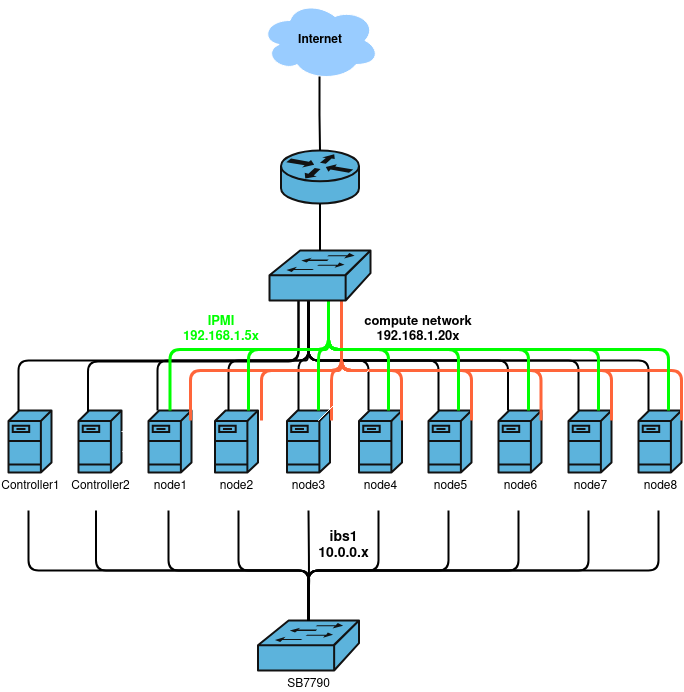
\includegraphics[width=0.8\textwidth]{assets/diagram.png}
    \caption{asd}
    \label{fig:diagram}
\end{figure}


\newpage

\subsection{Poloautomatická instalace}
\label{Skript}
Pro jednoduchost byla sepsána řada skriptů pro automatizování částí instalace celého systému OpenNebula, ovladačů pro InfiniBand\cite{InfiniBand}, MariaDB a Chrony. Jednotlivé kroky těchto skriptů budou vysvětleny v přůběhu návodu.

\begin{small}
\texttt{curl -fsSl https://raw.githubusercontent.com/KopyTKG/UJEP-LAB/refs/heads/Live/\\tools/full.sh | sudo bash}
\end{small}

\subsection{Nastavení síťového připojení}
\label{sitove nastaveni}
Pro jednoduchost nastavení použijeme jíž předinstalovanou aplikaci \textbf{nmcli}. Použití aplikace není nijak složité. V další sekvenci obrázků lze následovat jednoduché kroky pro nastavení interface ibs1 na statickou ip adresu.

Pozor \textit{controller} má jiné pojmenování síťového portu a to jest \textbf{\textit{ibp1s0}}.

\begin{verbatim}
[root@controller]# nmcli con mod ibs1 ipv4.addresses 10.0.0.1/23 ipv4.method manual
[root@controller]# nmcli con mod ibs1 connection.autoconnect yes
[root@controller]# nmcli con up ibs1
\end{verbatim}

\subsection{Nastavení SSH}
Generace klíče není nutná po instalace pomocí skriptu viz \ref{Skript}

Pro plnou funkci je nutno povolit komunikaci pro \textit{root} uživatele. Pro bezpečnost povolíme jen přihlášení pomocí klíče a pro je potřeba vygenerovat klíče přes příkaz \textit{ssh-keygen} s pomocí parametru \textit{-t ed25516}.
\begin{verbatim}
[root@controller]# ssh-keygen -t ed25519 -f /root/.ssh/id_ed25519 -N ""
\end{verbatim}

Z důvodu bezpečnosti nebudeme povolovat přihlášení uživatele root přes heslo a proto je nutno se manuálně přihlásit na každý systém a vytvořit soubor \textit{/root/.ssh/authorized\_keys} s obsahem veřejného klíče z \textit{controller} kde byl vytvořen.

\begin{small}
\texttt{[root@controller]\# cat /root/.ssh/id\_ed25519.pub}\\
\texttt{ssh-ed25519 AAAAC3NzaC1lZDI1NTE5AAAAIC3Qw1k8Qn1v8Qw2Zk1Qw2Zk1Qw2Zk1Qw2Zk1Qw2Zk1Qw2Zk1Q\\w2Zk1Qw2Zk1 root@controller}

\texttt{[root@nodeX]\# echo "ssh-ed25519 AAAAC3NzaC1lZDI1NTE5AAAAIC3Qw1k8Qn1v8Qw2Zk1Qw2Zk1Qw2Zk\\1Qw2Zk1Qw2Zk1Qw2Zk1Qw2Zk1Qw2Zk1 root@controller" \textgreater{}\textgreater{} /root/.ssh/authorized\_keys}
\end{small}

\newpage

\subsection{Přednastavení pro instalaci}
Pro možnost instalace s použitím IPoIB je nutno dodat názvy systémů (Hostname) do \textit{/etc/hosts} a to na všechny stroje kde soubor bude vypadat tak to
\begin{verbatim}
[root@controller]# vim /etc/hosts | nano /etc/hosts

127.0.0.1   localhost localhost.localdomain localhost4 localhost4.localdomain4
::1         localhost localhost.localdomain localhost6 localhost6.localdomain6

10.0.1.1  controller

10.0.0.1  node1
10.0.0.2  node2
10.0.0.3  node3
10.0.0.4  node4
10.0.0.5  node5
10.0.0.6  node6
10.0.0.7  node7
10.0.0.8  node8

192.168.1.201  Eth-node1
192.168.1.202  Eth-node2
192.168.1.203  Eth-node3
192.168.1.204  Eth-node4
192.168.1.205  Eth-node5
192.168.1.206  Eth-node6
192.168.1.207  Eth-node7
192.168.1.208  Eth-node8
\end{verbatim}

po nakonfigurování je nutno ověřit síťové spojení a to ze pomoci \textit{hostname} názvů uvedených v \textit{/etc/hosts}. Testu dosáhneme pomocí jednoduchého ping příkazu.

\begin{verbatim}
[user@controller]$ ping Eth-nodeX
\end{verbatim}

\subsection{Instalace Compute systémů}

\subsection{Základní instalace}

\subsubsection{Instalace NTP serveru}
Jako první krok musím zkontrolovat instalaci a konfigurace NTP serveru. Pro náš testovací cluster byly zvoleny NTS servery od CESNET\cite{CESNET} a to jest \textit{tik.cesnet.cz} a \textit{tak.cesnet.cz}. Pro kontrolu instalace stačí spustit instalaci pomocí příkazu.

\begin{verbatim}
$ sudo dnf install -y chrony
\end{verbatim}

\newpage

Po instalaci použijeme program \textit{tee} pro rychlé přepsáný konfigurace chrony. Tee přepíše celý soubor na následující konfiguraci.

\begin{verbatim}
$ tee /etc/chrony.conf > /dev/null <<EOF
server tik.cesnet.cz iburst
server tak.cesnet.cz iburst

sourcedir /run/chrony-dhcp
driftfile /var/lib/chrony/drift
makestep 1.0 3
rtcsync
keyfile /etc/chrony.keys
ntsdumpdir /var/lib/chrony
leapsectz right/UTC
logdir /var/log/chrony
EOF
\end{verbatim}

Dále jen nutno povolit NTP v firewall a restartovat službu pro znovu načtení konfigurace.
\begin{verbatim}
$ sudo firewall-cmd --permanent --add-service=ntp
$ sudo firewall-cmd --reload
$ sudo systemctl restart chronyd.service
\end{verbatim}

\subsubsection{Instalace SQL databáze}
Pro funk
\begin{verbatim}
$ sudo dnf install mariadb mariadb-server python3-PyMySQL -y
\end{verbatim}

Dále jen nutno přidat konfiguraci

\begin{verbatim}
$ tee /etc/my.cnf.d/openstack.cnf > /dev/null <<EOF
[mysqld]
#nutno pro propojeni IB a Eth (Dashboard a Compute)
bind-address = 0.0.0.0 

default-storage-engine = innodb
innodb_file_per_table = on
max_connections = 4096
collation-server = utf8_general_ci
character-set-server = utf8
EOF
\end{verbatim}

Jako poslední jíž jen spustit službu a dokončit základní konfiguraci

\begin{verbatim}
$ sudo systemctl enable mariadb.service --now
$ sudo mysql_secure_installation
\end{verbatim}

Heslo pro root uživatele (DB\_PASS) si zapište do tabulky viz.: Tabulka hesel \ref{fig:gen-pass-table}

\newpage
\subsubsection{Instalace RabbitMQ}
\subsubsection{Instalace Memcached}

\newpage
\section{Open Nebula}


\begin{figure}[!h]
    \centering
    \begin{tabular}{|l|l|}
    \hline
     \textbf{Název hesla} & \textbf{Heslo} \\
     \hline
     DB\_PASS & 3a81192d09bb454cc35afe06f1cafc5711dec572  \\
     DB\_Oneadmin & 4be5d88f91795e71dce8f4bd626423eef224b30b \\
     KEYSTONE\_DBPASS   & c7246b82ec9b8ca5a7a3fd9f82527e88e2cbc4e6 \\
     GLANCE\_DBPASS     & dca5717ca9bb55581b099e45619da1ffa690e4ce \\
     DASH\_DBPASS       &  \\
     NEUTRON\_DBPASS    & 564b8c564027a33d1cb2e6f724a7a61ca9b9cd0f \\
     NOVA\_DBPASS       & 0eb74ae1f47c0c8495bcf4db9c775a898bc4047b \\
     PLACEMENT\_DBPASS  & d30cfe364a80a7bb53bb758460f325c4292f3f3f \\
     ADMIN\_PASS        & ebf440559b2034e003a4603276ea057cd41ba52e \\
     USER\_PASS         & heslo \\
     GLANCE\_PASS       & 7434063c6875ae43ada80c7267b7437c61ab3845 \\
     DASH\_PASS         &  \\
     NEUTRON\_PASS      & 5b784b0a051a48b23edbd37ac8df53b00819d257 \\
     NOVA\_PASS         & 170b9b7265e0785412ac20cb2539bfde8e21f9bf \\
     PLACEMENT\_PASS    & b54867e5a60c03f0596bdf81f2226886af22e2d7 \\
     \hline
    \end{tabular}
    \label{fig:gen-pass-table}
\end{figure}

CREATE USER 'oneadmin' IDENTIFIED BY '4be5d88f91795e71dce8f4bd626423eef224b30b';
GRANT ALL PRIVILEGES ON opennebula.* TO 'oneadmin';
SET GLOBAL TRANSACTION ISOLATION LEVEL READ COMMITTED;



\begin{verbatim}
repo=$(yum repolist --disabled | grep -i -e powertools -e crb | awk '{print $1}' | head -1)
yum config-manager --set-enabled $repo && yum makecache
 cat << "EOT" > /etc/yum.repos.d/opennebula.repo
[opennebula]
name=OpenNebula Community Edition
baseurl=https://downloads.opennebula.io/repo/6.10/RedHat/$releasever/$basearch
enabled=1
gpgkey=https://downloads.opennebula.io/repo/repo2.key
gpgcheck=1
repo_gpgcheck=1
EOT

yum makecache

dnf install mariadb mariadb-server -y
systemctl enable mariadb.service --now
mysql_secure_installation 
mysql -u root -p
rpm -ivh https://dl.fedoraproject.org/pub/epel/epel-release-latest-9.noarch.rpm
yum -y install opennebula opennebula-fireedge opennebula-gate opennebula-flow opennebula-provision
sudo -u oneadmin /bin/sh
systemctl enable --now  opennebula opennebula-fireedge opennebula-gate opennebula-flow
oneuser show
firewall-cmd --add-port=2616/tcp --permanent
firewall-cmd --reload


\end{verbatim}
\newpage

\subsection{CEPH}

\begin{verbatim}
dnf config-manager --set-enabled crb

dnf install centos-release-ceph-reef -y
dnf install cephadm -y
dnf install ceph-common -y

firewall-cmd --add-port={8443,3000,9095,9093,9094,9100,9283}/tcp --permanent


\end{verbatim}

\subsubsection{Controller}

\begin{verbatim}
cephadm bootstrap --mon-ip 192.168.1.x # Ethernet port pro pripojeni po siti

ssh-copy-id -f -i /etc/ceph/ceph.pub root@*node1 - node8*

ceph orch host add nodeX 10.0.0.X # X = 1 - 8

ceph orch apply osd --all-available-devices
\end{verbatim}

\ukol{libvirt compute\_driver nova.conf} 
\ukol{ update httpd config for placement api}
\ukol{add nova-compute perms to python core}

\newpage

\subsubsection{V}


\newpage

\printbibliography

\end{document}
